\documentclass[a4paper, 10pt]{article}

\usepackage{wrapfig}
\usepackage{listings}
%Math
\usepackage{amsmath}
\usepackage{amsfonts}
\usepackage{amssymb}
\usepackage{amsthm}
\usepackage{ulem}
\usepackage{textcomp}


%PageStyle
\usepackage[german]{babel}
\usepackage{fontenc}
\usepackage{fancyhdr, graphicx}
\usepackage{fullpage}
\usepackage{graphicx}
\usepackage{textcomp}
\usepackage{fancyhdr} %for header/footer
\usepackage{wrapfig}


\newcommand{\Bold}[1]{\textbf{#1}} %Boldface
\newcommand{\Kursiv}[1]{\textit{#1}} %Italic

%Metadata
\title{Betriebssysteme Test 2}
\author{Jan F\"assler}
\date{2. Semester (FS 2012)}
\fancyfoot[C]{If you use this documentation for a exam, you should offer a beer to the authors!}

%Config
\renewcommand{\headrulewidth}{0pt}
\setlength{\headheight}{15.2pt}
\pagestyle{plain}

\begin{document}
% Titelbild
\maketitle
\thispagestyle{fancy}

\newpage


% Inhaltsverzeichnis
\pagenumbering{Roman}
\tableofcontents	  	


\newpage
\setcounter{page}{1}
\pagenumbering{arabic}

\section{Parallelit\"at - Nebenl\"aufigkeit}
\subsection{Einleitung}
Falls ein Rechner mehrere Prozesse parallel verarbeiten kann (Multi-Tasking), so f\"uhrt er jeden Prozess als separate Aktivit\"at aus. Diese Prozesse können unabh\"angig voneinander ablaufen (Nebenl\"aufigkeit), m\"ussen jedoch synchronisiert werden, da bestimmte Ressourcen (insbesondere die CPU) gemeinsam genutzt werden. Stehen mehrere CPUs zur Verf\"ugung, können Prozesse parallel ablaufen, jedoch weiterhin mit Synchronisation und Wartezust\"anden bei gemeinsam genutzten Ressourcen. Werden Threads innerhalb eines Prozess-Adressraums eingesetzt, gilt diese Aussage sinngem\"ass auch f\"ur jeden Thread innerhalb eines Prozesskontexts.

\subsection{Der Sheduler}
Der Scheduler teilt Prozessen Rechenzeit zu und sequentialisiert damit die nebenl\"aufige Ausf\"uhrung von Prozessen oder Threads auf einer oder mehreren CPUs. Bei gen\"ugender Performance des Systems geschieht dies so rasch, dass f\"ur den Benutzer der Eindruck der Parallelit\"at entsteht. Neben der Ressourcenauslastung beeinflusst die Scheduling-Strategie den Grad der Quasi-Parallelit\"at.

\subsection{Pre-emption}
Prozesse können in Unix zu fast jeder Zeit unterbrochen werden:
\begin{itemize}
	\item freiwillig durch Systemaufruf mit Wartezustand oder Abgabe der CPU (sleep, wait)
	\item ungeplant durch den Scheduler auf Basis von Priorisierung und Ressourcenverbrauch oder nach Ablauf der Zeitscheibe
	\item ungeplant durch asynchronen Events (z.B. Interrupts, die durch den gerade laufenden Prozess behandelt werden m\"ussen)
\end{itemize}
Ein Prozess muss seinen Ausf\"uhrungskontext unter- brechen, abspeichern, zum neuen Kontext wechseln, im neuen Kontext ablaufen, den alten Kontext wiederherstellen und neu starten können (Aufgabe des Kernels). Behandelt der Prozess im Programmcode Ausnahmen selbst (z.B. Signale), muss der Programmierer selbst f\"ur die Konsistenz von Variablen und Zust\"anden sorgen.

\subsection{Synchronisation}
\subsubsection{Das Problem der Synchronisierung}
5 Personen sitzen am Tisch, zwischen den Personen liegen 5 St\"abchen. Zum Essen benötigt jede Person 2 St\"abchen.
\begin{description}
	\item[Warten] Griff in‘s Leere
	\item[Synchronisation] Gleichzeitiger Zugriff
	\item[Deadlock] jede Person nimmt das rechte St\"abchen und wartet auf das linke
	\item[Starvation] alle Personen sollen in sinnvolle Frist essen
\end{description}

\subsubsection{Synchronisation}
Zwischen Kernel und Prozessen:
\begin{itemize}
	\item Signalisierung	
	\item Schlaf-/Wartezustand des Prozesses
	\item Aufwecken \& Scheduling
\end{itemize}
Zwischen Prozessen:
\begin{itemize}
	\item Einseitige Synchronisation
	\item Mehrseitige Synchronisation
	\item Gegenseitiger Ausschluss aus kritischen Abschnitten
\end{itemize}

\subsection{Synchronisationsmittel}

\subsubsection{Benachrichtigung \& Warten}
\begin{itemize}
	\item Prozess wartet aktiv auf das Eintreffen einer Nachricht (busy waiting)
	\item Prozess wartet(schl\"aft) auf das Eintreffen eines Wecksignals (typisiert) – der Signal-Mechanismus von Unix weckt dann (via den Kernel / Scheduler) alle auf dieses Ereignis wartenden Prozesse
\end{itemize}

\subsubsection{Locks/Schlossvariablen}
\begin{itemize}
	\item Im Dateisystem (Lockfile, Lock-Bits im Superblock)
	\item Im Speicher (Lock Bits, gemeinsame Variablen)
	\item Modell: der Prozess pr\"uft zyklisch auf Zustands\"anderung des Bits / der Variablen und modifiziert das Bit bzw. die Variable, falls erlaubt.
	\item Problem: meist keine atomare Operation wegen jederzeitiger Unterbrechbarkeit, es kann daher zu Problemen kommen, wenn die Implementation nicht durch unteilbare CPU-Instruktionen unterst\"utzt wird.
\end{itemize}

\subsubsection{Ereignisz\"ahler}
\begin{itemize}
	\item Variante eines Locks, welches durch eine Z\"ahlervariable (z.B. in einem Shared Memory Segment) implementiert wird.
	\item Sinnvoll, wenn mehrere Prozesse zu synchronisieren sind, z.B. maximale Anzahl quasiparalleler Leseprozesse auf einer Datenbank wegen Performance-Garantien.
	\item Gleiches Problem der unterbrechbaren, nicht atomaren Operation wie bei Locks, benötigt daher \"ahnliche Schutzmechanismen.
\end{itemize}

\subsubsection{Petri-Netze}
Modellierung von nebenl\"aufigen Systemen und ihrer Synchronisation
\begin{itemize}
	\item Stellen = Kreis
	\item Transitionen = Rechteck
	\item Marken = Punkt
	\item Schaltregeln = alle vorausgehenden Stellen enthalten mind. 1 Marke, alle nachfolgenden Stellen erhalten eine Marke
\end{itemize}

\subsubsection{Dijkstra Semaphore}
\begin{itemize}
	\item Modul/Kapsel mit gesch\"utzter Statusvariablen
	\item Bereitstellung von Operationen f\"ur:
		\begin{itemize}
				\item Initialisierung
				\item Eintritt/Signalisierung (P)
				\item Austritt/Freigabe (V)
				\item Deallokation
		\end{itemize}
	\item Typen:
		\begin{itemize}
			\item Bin\"ar	
			\item Z\"ahler
			\item Set / Array
		\end{itemize}
	\item Implementierung: atomare CPU-Instruktion oder kurzzeitige Erhöhung des Interrupt-Levels
\end{itemize}

\subsubsection{Barrier}
Die fehlerhafte Programmierung eines wechselseitigen Ausschlusses mit Semaphoren kann zu signifikanten Fehlern f\"uhren - neues Sprachkonstrukt MONITOR ohne explizite Programmierung von P und V Operationen – stattdessen Generierung durch den Compiler .
\begin{itemize}
	\item Modul, welches Daten und Methoden/Prozeduren enth\"alt.
	\item Aufruf des Monitor Entry durch beliebig viele Prozesse; Garantie des wechselseitigen Ausschlusses
	\item Prozeduren/Methoden eines Monitors können auf globale Daten zugreifen, die lokalen Daten des Monitors sind aber von aussen nicht zug\"anglich
	\item Im Innern eines Monitors ist es ggf. nötig, dass eine Aktivit\"at wartet. Eine solche Aktivit\"at wird durch den Monitor aus dem Monitor ausgelagert. Auf diese Weise bleibt der Monitor nicht blockiert und eine andere Aktivit\"at kann in den Monitor eintreten. Falls eine andere Aktivit\"at den Wartenden befreit, so kann diese, sobald der Monitor frei ist, diesen wieder betreten.	
\end{itemize}

\subsubsection{Rendezvous}
\begin{itemize}
	\item Synchronisation von entfernten Prozedurauf- rufen (remote procedure calls)
	\item Der Prozedur-Aufrufer wird blockiert, bis die ent- fernte Prozedur ausgef\"uhrt wurde
	\item Der Prozedur-Anbieter bleibt blockiert, bis eine seiner Prozeduren aufgerufen wird.
	\item Operationen:
		\begin{itemize}
			\item Rendenzvous anbieten (Anbieter)
			\item Rendezvous beantragen (Aufrufer) - Warteschlange
			\item Rendezvous annehmen (Anbieter) - erster Aufrufer
			\item Rendezvous ausf\"uhren \& Resultat melden (Anbieter)
		\end{itemize}
\end{itemize}

\subsection{Deadlock Erkennung und Vermeidung/Behebung}
Deadlocks treten auf, wenn:
\begin{itemize}
	\item die umstrittenen Ressourcen nur exklusiv nutzbar sind,
	\item die umstrittenen Ressourcen nicht entzogen werden können,
	\item die Belegung von Ressourcen schon möglich ist, auch wenn auf die Zuweisung weiterer Ressourcen gewartet werden muss,
	\item eine zyklische Kette von Prozessen auftritt, in der jeder Prozess mindestens eine Ressource besitzt, die der n\"achste Prozess in der Kette benötigt.
\end{itemize}
Gegenmassnahmen:
\begin{itemize}
	\item Sicherstellen, dass immer eine der Deadlock-Bedingungen nicht erf\"ullt ist (Regeln f\"ur die Nutzung / erzwungene Freigabe etc).
	\item Zuk\"unftigen Ressourcenbedarf der Prozesse analysieren und Zust\"ande erkennen/verbieten, die zu Deadlocks f\"uhren.
	\item Bereits eingetretenden Deadlock erkennen und auflösen.
\end{itemize}


\newpage
\section{Verteilte vs. monolithische Betriebssysteme}
\subsection{Strategien / Varianten}
\begin{itemize}
	\item Hardware / Software / Benutzung
	\item Client-Server-System: Viele Clients greifen auf einen oder mehrere Server bzw. Services zu.
	\item Verteiltes Dateisystem: Ein \"uber mehrere Server verteiltes virtuelles Dateisystem steht Clients zur transparenten Benutzung zur Verf\"ugung.
	\item Netzwerkf\"ahiges Betriebssystem: das Betriebssystem stellt system\"ubergreifende Funktionalit\"at zur Verf\"ugung.
	\item Verteiltes Betriebssystem: Das Betriebssystem selbst ist verteilt, f\"ur Benutzer und Anwendungen ist dies nicht sichtbar.
	\item Verteilte Anwendung: Durch die Programmierung der Anwendung wird das verteilte System erstellt – das Programm muss in der Regel die Verteillogik kennen.
\end{itemize}

\subsection{Vorteile \& Risiken}

\subsubsection{Vorteile}
\begin{itemize}
	\item Verteilung versus Parallelit\"at
	\item Lastverteilung
	\item Leistungssteigerung
	\item Skalierbarkeit/Flexibilit\"at
	\item Sicherheit/Zuverl\"assigkeit/Verf\"ugbarkeit
	\item Preis/Leistungbzw.Kostenreduktion
	\item Gemeinsame Datennutzung
	\item Gemeinsame Nutzung teurer Peripherie
	\item Applikatorische Verteilung
\end{itemize}

\subsubsection{Risiken}
\begin{itemize}
	\item Erhöhte Komplexit\"at
	\item Erschwerte Fehlersuche	
	\item Verl\"angerte Abh\"angigkeitsketten
	\item Sicherheitsdispositiv wird aufwendiger
	\item Nicht alle Subsysteme eignen sich f\"ur die Verteilung
	\item Sicherstellung der Konsistenz und Synchronisation
\end{itemize}

\subsection{Anforderungen an verteilte Betriebssysteme}
\begin{itemize}
	\item Gemeinsamer Kernel Code und System Calls
	\item Gemeinsam genutzter Hauptspeicher
	\item Gemeinsames Prozess-Steuersystem
	\item Gemeinsames Dateisystem
	\item Gemeinsame Interprozess-Kommunikation
	\item Gemeinsame Ausnahmebehandlung
	\item Gemeinsame Synchronisationsmechanismen
	\item Gemeinsames System Management
	\item Spezialisierte Funktionen f\"ur das Management der Verteilung
	\item Transparente Benutzerschnittstelle
\end{itemize}

\subsubsection{Transparenz}
\begin{description}
	\item[Ortstransparenz:] \hfill \\ Der Ort der genutzten Ressourcen / erbrachten Dienste ist f\"ur den Anwender nicht sichtbar.
	\item[Migrationstransparenz:] \hfill \\ Ressourcen können verlagert werden, ohne dass sich ihr Name bzw. ihre Nutzung ver\"andert.
	\item[Replikationstransparenz:] \hfill \\ Anwender können nicht erkennen, wie viele Instanzen es gibt.
	\item[Nebenl\"aufigkeitstransparenz:] \hfill \\ mehrere Anwender können die Ressourcen automatisch gemeinsam und unabh\"angig voneinander nutzen.
	\item[Parallelit\"atstransparenz:] \hfill \\ Aktivit\"aten können parallel bzw. Nebenl\"aufig ausgef\"uhrt werden, ohne dass der Anwender es bemerkt.
\end{description}

\subsubsection{Flexibilit\"at}
Services sollen dynamisch an den Bedarf anpassbar sein, entweder durch administrative Eingriffe oder durch Eigenkonfiguration zur Laufzeit. \"anderungen sollen keinen kompletten Neustart des verteilten Systems erfordern.

\subsubsection{Zuverl\"assigkeit}
\begin{itemize}
	\item Erhöhte Zuverl\"assigkeit gegen\"uber Einzel- systemen trotz additiver Ausfallwahrschein- lichkeiten
	\item End-zu-End Verf\"ugbarkeit statt Komponentenverf\"ugbarkeit.
	\item Sicherheit – gleiche Richtlinien \& Umsetzung im gesamten verteilten System.
	\item Fehlertolerenz
	\item Automatisches Recovery von Komponenten.
\end{itemize}

\subsubsection{Performance}
\begin{itemize}
	\item Verteilungs- und Kommunikations- Mehraufwand muss den Aufwand wert sein
	\item Wiederholbarkeit / Determinismus von Leistungsindikatoren.
	\item Abh\"angigkeit von nicht direkt kontrollier- baren Komponenten
	\item End-zu-End Performance statt Komponenten-Performance.
\end{itemize}

\subsubsection{Skalierbarkeit}
Angebotsseite:
\begin{itemize}
	\item Statische oder dynamische Zuf\"ugung / Weg- nahme von Servern.
	\item Verrechnung: Durchschnitt oder peaks?
	\item Vermeiden von „Flaschenh\"alsen“ durch zu starke Serialisierung.
\end{itemize}
Dienstnehmerseite:
\begin{itemize}
	\item Nicht vorhersagbare Anzahl Dienstnehmer.
	\item Einhaltung von Dienstg\"utegarantien
\end{itemize}

\subsection{Synchronisation in verteilten Systemen}
\begin{description}
	\item[Zeitsynchronisation] \hfill
		\begin{itemize}
			\item Absolut
			\item Relativ
			\item Vorstellen ist einfacher als R\"uckstellen
		\end{itemize}
	\item[Gegenseitiger Ausschluss \"uber Systemgrenzen] \hfill
		\begin{itemize}
			\item Zentraler Algorithmus (mit Redundanz)
				\begin{itemize}
					\item Zuverl\"assig, berechenbar
					\item Starke Serialisierung
				\end{itemize}
			\item Verteilter Algorithmus
				\begin{itemize}
					\item Zeitliche Ordnung im Gesamtsystem
					\item Getimte Nachricht an alle Prozesse und Warten auf Best\"atigung 
				\end{itemize}
			\item Token Ring Algorithmus
				\begin{itemize}
					\item Explizite Erlaubnis zum Zugriff in vordefinierter Reihenfolge
					\item Suboptimale Ressourcennutzung / Wartezeiten
				\end{itemize}
		\end{itemize}
\end{description}

\newpage
\section{Sicherheitsaspekte im Betriebssystem}
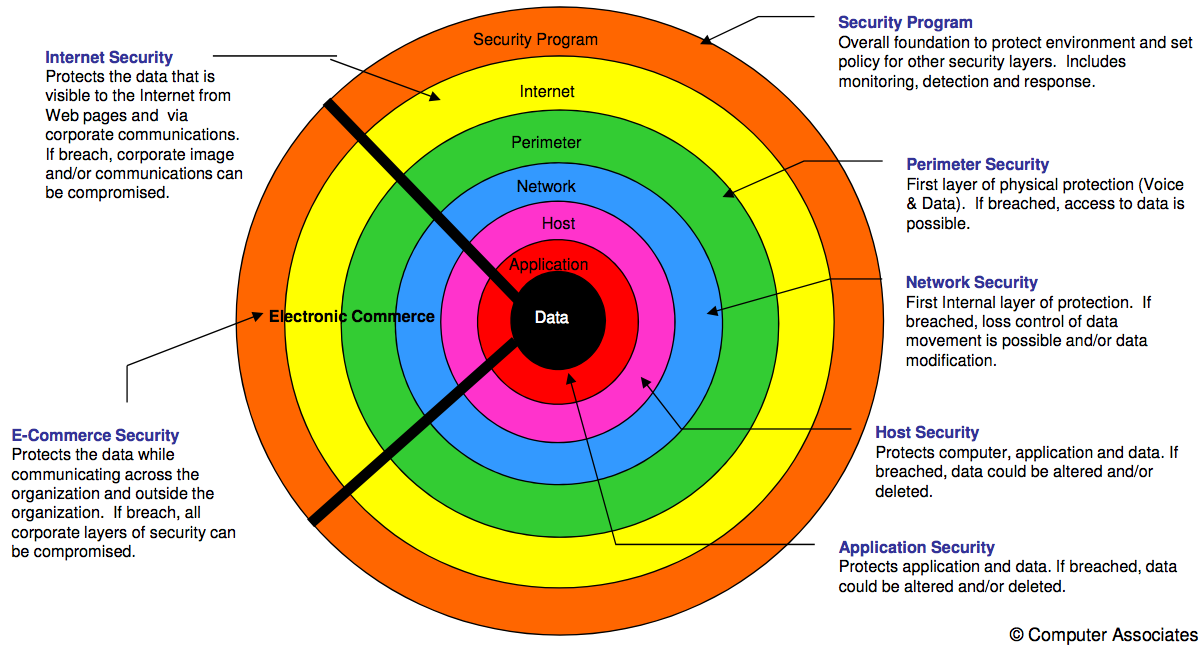
\includegraphics[scale=0.35]{onion_security.png}
\subsection{Typische Schwachstellen}
\begin{itemize}
	\item Lieferwege (physisch, aber vor allem elektronisch)
	\item Software-Voreinstellungen(Defaults)
	\item Funktionale Fehler der Software / Ausnutzbarkeit von Nebeneffekten
	\item Nicht getestete oder nicht autorisierte \"anderungen
	\item Fremd-/Fernzugriffe oder Auslagerung aus dem Sicherheits-Kontext
	\item Der Benutzer
	\item Der Administrator
\end{itemize}
\subsection{Ursachen}
\begin{itemize}
	\item Komplexes Zusammenwirken verschiedener Effekte
	\item Ungerechtfertigtes Vertrauen
	\item Gutwilligkeit der Beteiligten
	\item Fehlerhafte Ausf\"uhrung und/oder Kontrolle
	\item Böswilligkeit / Vorsatz
\end{itemize}
\subsection{Sicherheits-Management}
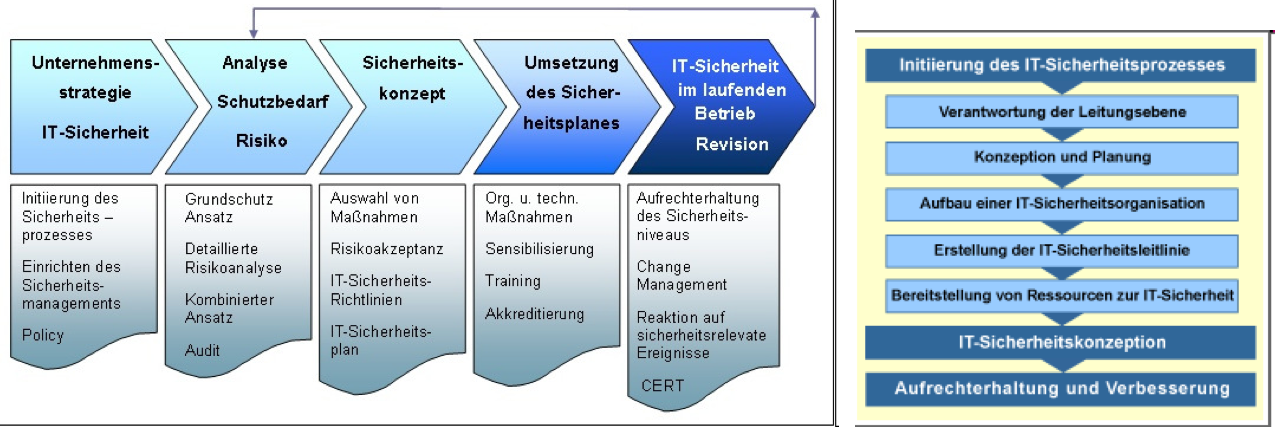
\includegraphics[scale=0.35]{sicherheits_management.png}
\subsection{Risiko-Management}
\begin{itemize}
	\item Die wissentliche oder unwissentliche Akzeptanz einer Verlustwahrscheinlichkeit und möglichen Schadenhöhe.
	\item Risiko-Management durch:
		\begin{itemize}
			\item Analyse
			\item Vermeidung (nur bedingt möglich, ...)
			\item \"Ubertragung (Versicherung, Werkschutz,...)
			\item Begrenzung (pr\"aventive Massnahmen,...)
			\item Akzeptanz (formaler, dokumentierter Willensakt)
			\item Ignoranz (wegschauen,...)
		\end{itemize}
\end{itemize}
Meist gibt es eine Mischung der Massnahmen, abh\"angig vom Risikotyp, der Risikokultur, den Kostenfolgen usw.
\end{document}
